\documentclass[border=2pt]{standalone}
% Computer Modern, the font of the handouts (pdflatex)
\usepackage{amsmath}
\usepackage{tikz}
\usepackage{pgfplots}
\pgfplotsset{compat=1.18}
\usetikzlibrary{arrows.meta,calc}
\definecolor{cA}{HTML}{2A78D6}
\definecolor{cB}{HTML}{EB6834}
\definecolor{cC}{HTML}{1BAF7A}
\definecolor{cD}{HTML}{EDA100}
\definecolor{cE}{HTML}{E87BA4}
\definecolor{nodeblue}{HTML}{1565C0}
\definecolor{linkgray}{HTML}{546E7A}
\definecolor{lightgray}{HTML}{CFD8DC}
\definecolor{txt}{HTML}{263238}
\definecolor{band}{HTML}{EEEEEE}
\definecolor{uUnused}{HTML}{BDBDBD}
\definecolor{uLow}{HTML}{2E7D32}
\definecolor{uMid}{HTML}{F9A825}
\definecolor{uHigh}{HTML}{EF6C00}
\definecolor{uFull}{HTML}{C62828}
\definecolor{uOver}{HTML}{7B1FA2}
\tikzset{
  nd/.style={circle, fill=nodeblue, draw=white, line width=0.7pt, minimum size=#1, inner sep=0pt},
  nd/.default=3.2mm,
  nlab/.style={font=\footnotesize\bfseries, text=txt, inner sep=1pt},
  lbl/.style={font=\scriptsize, text=txt, fill=white, fill opacity=0.85, text opacity=1, inner sep=0.7pt},
  arr/.style={-{Stealth[length=1.9mm, width=1.5mm]}},
}
\pgfplotsset{
  lab/.style={
    scale only axis, axis lines*=left, grid=major, grid style={black!12},
    tick label style={font=\small}, label style={font=\normalsize},
    ylabel style={align=center},
    legend style={draw=none, fill=none, font=\small},
    legend cell align=left, tick align=outside, axis line style={black!60},
    every axis plot/.append style={line width=1.1pt},
  },
  % the series differ in color, marker and line style (readable in black and white);
  % the second series has hollow markers, visible where the two curves overlap
  s1/.style={cA, solid, mark=*, mark size=1.7pt},
  s2/.style={cB, densely dashed, mark=square*, mark size=1.6pt, mark options={solid, fill=white}},
  s3/.style={cC, dashdotted, mark=diamond*, mark size=2.1pt, mark options={solid}},
  s4/.style={cD, densely dotted, mark=triangle*, mark size=2.1pt, mark options={solid, fill=white}},
  s5/.style={cE, dashed, mark=triangle*, mark size=2.1pt, mark options={solid, rotate=180}},
  ebars/.style={error bars/.cd, y dir=both, y explicit,
    error bar style={solid, line width=0.9pt}, error mark options={solid, rotate=90, mark size=2.2pt}},
}
\begin{document}
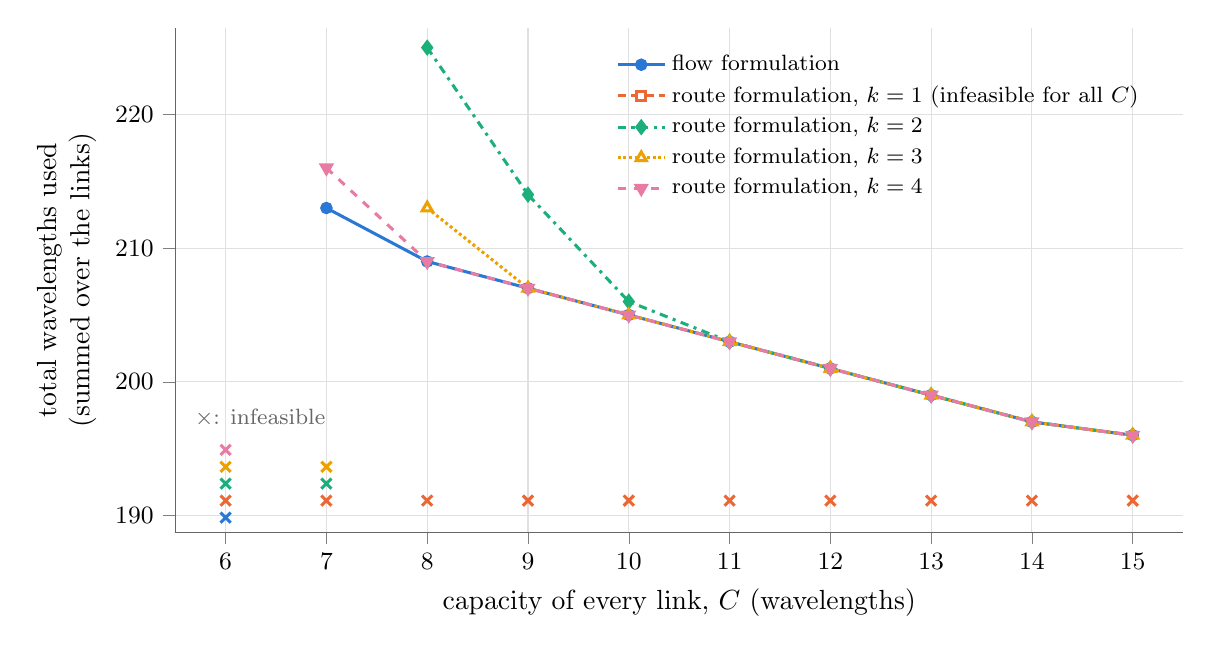
\begin{tikzpicture}\begin{axis}[lab, width=128mm, height=64mm, xmin=5.5, xmax=15.5, ymin=188.75, ymax=226.45, xtick={6,7,8,9,10,11,12,13,14,15}, xlabel={capacity of every link, $C$ (wavelengths)}, ylabel={total wavelengths used\\(summed over the links)}, legend pos=north east, legend style={font=\footnotesize}]
\addplot[s1] coordinates {(7,213) (8,209) (9,207) (10,205) (11,203) (12,201) (13,199) (14,197) (15,196)};
\addlegendentry{flow formulation}
\addlegendimage{s2}
\addlegendentry{route formulation, $k = 1$ (infeasible for all $C$)}
\addplot[s3] coordinates {(8,225) (9,214) (10,206) (11,203) (12,201) (13,199) (14,197) (15,196)};
\addlegendentry{route formulation, $k = 2$}
\addplot[s4] coordinates {(8,213) (9,207) (10,205) (11,203) (12,201) (13,199) (14,197) (15,196)};
\addlegendentry{route formulation, $k = 3$}
\addplot[s5] coordinates {(7,216) (8,209) (9,207) (10,205) (11,203) (12,201) (13,199) (14,197) (15,196)};
\addlegendentry{route formulation, $k = 4$}
\addplot[s1, only marks, mark=x, mark size=2.6pt, line width=1.1pt, forget plot] coordinates {(6,189.84)};
\addplot[s2, only marks, mark=x, mark size=2.6pt, line width=1.1pt, forget plot] coordinates {(6,191.11) (7,191.11) (8,191.11) (9,191.11) (10,191.11) (11,191.11) (12,191.11) (13,191.11) (14,191.11) (15,191.11)};
\addplot[s3, only marks, mark=x, mark size=2.6pt, line width=1.1pt, forget plot] coordinates {(6,192.38) (7,192.38)};
\addplot[s4, only marks, mark=x, mark size=2.6pt, line width=1.1pt, forget plot] coordinates {(6,193.64) (7,193.64)};
\addplot[s5, only marks, mark=x, mark size=2.6pt, line width=1.1pt, forget plot] coordinates {(6,194.91)};
\node[font=\footnotesize, text=black!60, anchor=south west] at (rel axis cs:0.01,0.19) {$\times$: infeasible};
\end{axis}\end{tikzpicture}
\end{document}
